\title{Chapter 2 Solutions}
\author{Sidhanth Holalkere}
\documentclass{article}

\usepackage[margin=1in]{geometry}
\usepackage{amsmath}
\usepackage{graphicx}
\graphicspath{{./}}

\begin{document}
\maketitle

\begin{enumerate}
    \item In $\epsilon$-greedy action selection, for the case of two actions and $\epsilon = 0.5$, what is the probability that the greedy action is selected.
    \begin{itemize}
        \item At the start, there is a $0.5$ chance that we immediately select the greedy action. If we don't select the greedy action, we randomly choose one of the two actions uniformly. The probability of randomly choosing the greedy action is $0.5 \times 0.5 = 0.25$. Therefore, the total probability that the greedy action is selected is $0.5 + 0.25 = 0.75$
    \end{itemize}

    \item \emph{Bandit example} Consider a $k$-armed bandit problem with $k=4$ actuibsm debited 1m 2m 3m abd 4, Consider applying to this problem a bandit algorithm using $\epsilon$-greedy action selection, sample average action-value estimates, and initial estimates of $Q_1(a) = 0$, for all $a$. Suppose the initial sequence of actions and rewards is $A_1 = 1$, $R_1 = -1$, $A_2 = 2$, $R_2 = 1$, $A_3 = 2$, $R_3 = -2$, $A_4 = 2$, $R_4 = 2$, $A_5 = 3$, $R_5 = 0$. On some of thesesteps the $\epsilon$ case may have occurred, causing a action to be selected at random. On which time steps did this definitely occur? On which time steps could this possibly have occurred?
    \begin{itemize}
        \item Starting at the beginning, $A_1$ could have been either since we don't know what the greedy action is yet. $A_2$ could have also been either since we still dont know what the greedy action is yet. $A_3$ definitely was an $\epsilon$ case since otherwise it would've chosen $2$ which has the highest $Q$ for now. $A_4$ could be either since it selected the greedy action (which could also have been randomly selected). And finally, $A_5$ is an $\epsilon$ step since it didn't choose the greedy action of $2$.
    \end{itemize}

    \item In the comparison shown in Figure 2.2, which method will perform best in the long run in terms of cumultive reward and probability of selecting the best action? How much better will it be? Express your answer quantitatively.
    \begin{itemize}
        \item Using $\epsilon=0.01$ will perform better in the long run since once the algorithm's action-values approach their true values, it will pick the greedy (best) option around $9\%$ more often than if you use $\epsilon=0.1$.
    \end{itemize}

    \item If the step-size parameters, $\alpha_n$, are not constant, then the estimate $Q_n$ is a weighted average of previously received rewards with a weighting different from that given by (2.6). What is the weighting on each prior reward for the general case, analogous to (2.6), in terms of the sequence of step-size parameters?
    \begin{itemize}
        \item \begin{align}
            Q_{n+1} &= Q_n + \alpha_n[R_n - Q_n] \\
            &= \alpha_n R_n + (1 - \alpha_n) Q_n \\
            &= \alpha_n R_n + (1 - \alpha_n)[\alpha_{n-1} R_{n-1} + (1 - \alpha_{n-1}) Q_{n-1}] \\
            &= \alpha_n R_n + (1 - \alpha_n)\alpha_{n-1} R_{n-1} + (1 - \alpha_n)(1 - \alpha_{n-1}) Q_{n-1} \\
            &= \alpha_n R_n + (1 - \alpha_n)\alpha_{n-1} R_{n-1} + (1 - \alpha_n)(1 - \alpha_{n-1}) \alpha_{n - 2}R_{n-2} + \\&... + (1-\alpha_n)(1-\alpha_{n-1})...(1-\alpha_2)\alpha_1 R_1 +\\& (1-\alpha_n)(1-\alpha_{n-1})...(1-\alpha_1)Q_1  \\
            &= \left( \prod^{n}_{i=1}(1-\alpha_i) \right) Q_1 + \sum^{n}_{i=1} \left(\left( \prod^{n}_{j=i+1}(1-\alpha_j) \right)\alpha_{i} R_i \right)
        \end{align}
    \end{itemize}

    \item Design and conduct and experiment to demonstrate the difficulties that sample-average methods have for nonstationary problems. Use a modified version of the 10-armed testbed in which all the $q_*(a)$ start out equal and then take independent random walks (say by adding a normally distributed increment with mean zero and standard deviation 0.01 to all the $q_*(a)$ on each step). Prepare plots like Figure 2.2 for an action-value method using sample averages, incrementally computed, and another action-value method using a constant step-size parameter, $\alpha=0.1$. Use $\epsilon=0.1$ and longer runs, say of 10,000 steps.
    \begin{itemize}
        \item See 2-2.py and Figure 1 and Figure 2 
        \begin{figure}[h]
            \caption{The return of models using either sample-averages to calculate $Q$ or a constant step-size (exponentially weighted average). The graph represents the average of 100 runs each.}
            \centering
            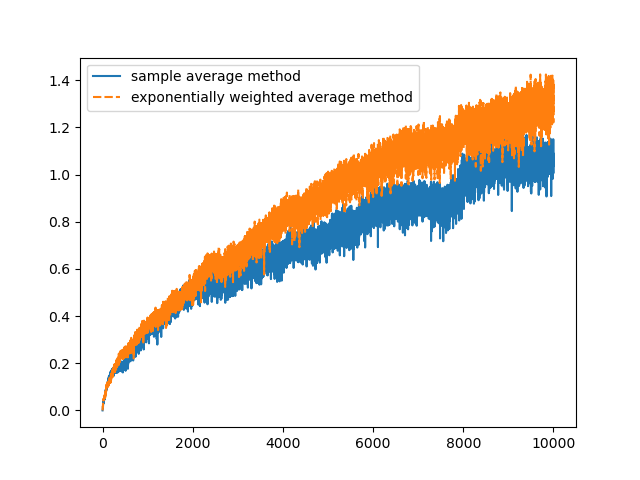
\includegraphics[scale=0.75]{figure-1.png}
        \end{figure}
        \begin{figure}[h]
            \caption{The percentage of choosing the optimal action of models using either sample-averages to calculate $Q$ or a constant step-size (exponentially weighted average). The graph represents the average of 100 runs each.}
            \centering
            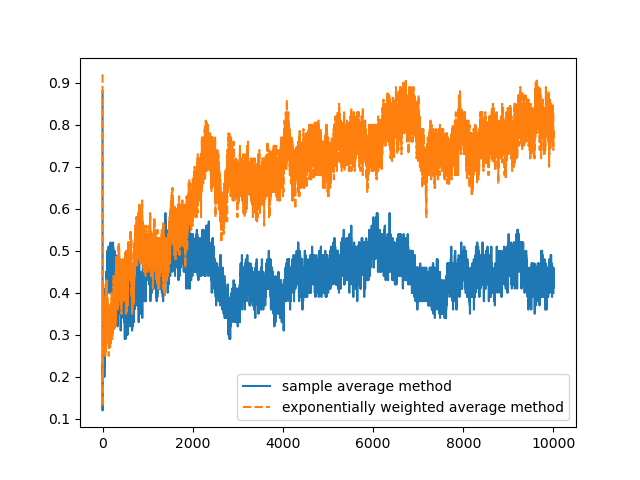
\includegraphics[scale=0.75]{figure-2.png}
        \end{figure}
    
    \end{itemize}

    \item \emph{Mysterious Spikes} The results shown in Figures 2.3 should be quite reliable because they are averages over 2000 individual, randomly chosen 10-armed bandit tasks. Why, then, are there oscillations and spikes in the early part of the curve for the optimistic method? In other words, what might make this method perform particularly better worse, on average, on particular early steps?
    \begin{itemize}
        \item Since the initial action-value predictions are optimistic, it takes longer for them to get closer to the true values, and therefore the algorithm spends more time thinking each action is "optimal" before identifying the truly optimal action. This makes it perform worse, on average, than using neutral action-values in earlier steps for the same reason.
    \end{itemize}

\end{enumerate}

\end{document}